% Nama Kelompok : Kelompok 2
% Kelas : D4 TI 1A
% 1. Kadek Diva Krishna Murti (1174006)
% 2. Duvan Silalahi (1174011)
% 3. Oniwaldus (1174005)
% 4. Choirul Anam (1174004)
% 5. Sri Rahayu (1174015)
% 6. Ilham Habibi (1174028)

\section{Pengertian}


Menurut F. Djuandi dalam bukunya yang berjudul "Pengenalan Arduino" \cite{djuandi2011pengenalan} IDE merupakan singkatan dari Integrated Development Environment atau lingkungan terintegrasi yang digunakan untuk melakukan pengembangan. Dikatakan sebagai lingkungan karena melalui software inilah dilakukan pemrograman Arduino untuk melakukan fungsi - fungsi yang ditanamkan melalui sintaks pemrograman. IDE ini disediakan gratis dan bisa didapatkan secara langsung pada halaman resmi arduino yang bersifat open source. IDE ini juga sudah mendukung berbagai sistem operasi populer saat ini seperti Windows, Mac, dan Linux. Arduino menggunakan bahasa pemrograman sendiri yang menyerupai bahasa C. Pada bahasa pemrograman Arduino (Sketch) telah dilakukan beberapa perubahan untuk memudahkan para pemula dalam melakukan pemrograman dari bahasa aslinya. Sebelum dijual ke pasaran, IC microcontroller Arduino telah ditanamkan suatu program bernama Bootlader yang berfungsi sebagai penengah antara compiler Arduino dengan microcontroller.



\section{Proses Instalasi}

\begin{enumerate}
\item Pertama unduh terlebih dahulu installer IDE Arduino di https://www.arduino.cc/en/Main/Software. Pada halaman tersebut ada tiga macam installer yang dapat diunduh sesuai dengan Operating System yang kita pakai.
\break
\centerline{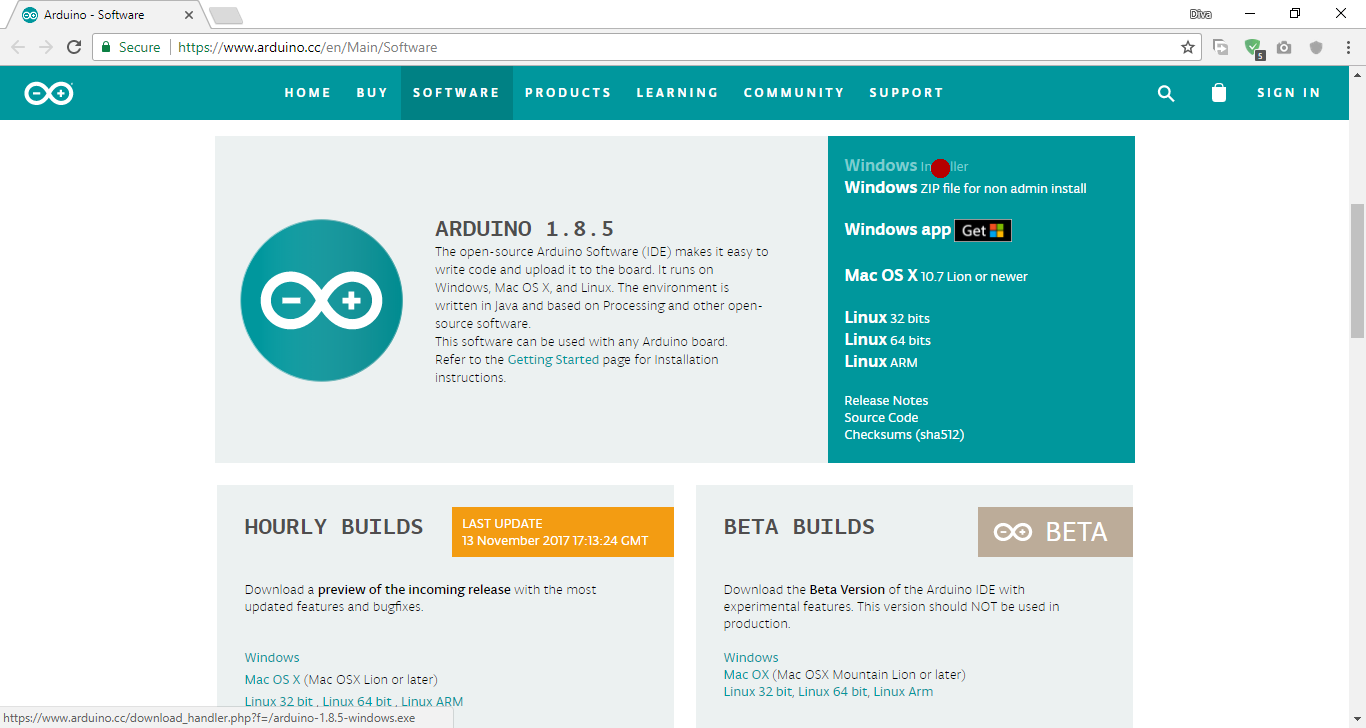
\includegraphics[width=0.9\textwidth]{figures/aride8.png}}
\item Kemudian pada halaman tersebut ada dua pilihan apakah kita ingin berkontribusi dengan memberikan uang sesuai dengan nominal yang tertera atau hanya mengunduh saja. Disini kita klik `Just Download' dan proses mengunduh dimulai.
\break
\centerline{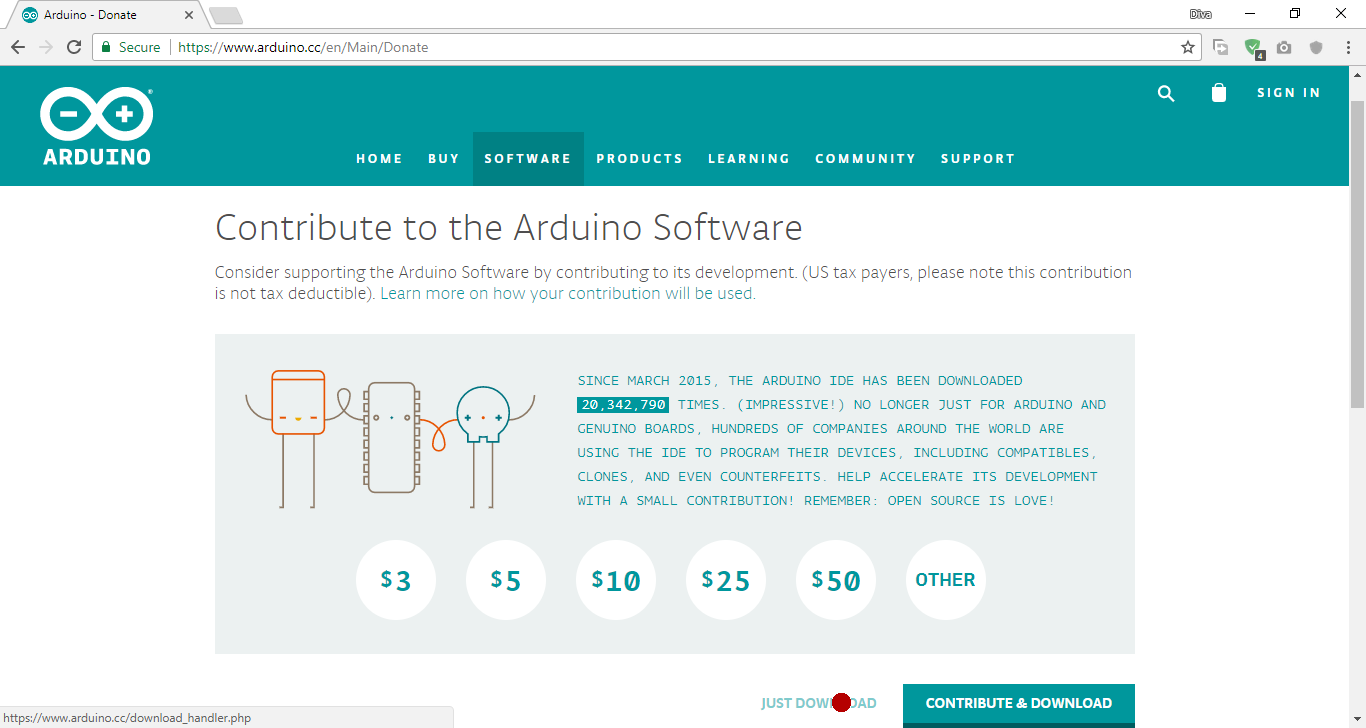
\includegraphics[width=0.9\textwidth]{figures/aride9.png}}
\item Setelah file installer telah selesai di unduh, lalu jalankan installer tersebut. Selanjutnya akan muncul jendela `Arduino Setup: License Agreement'. Lalu klik tombol `I Agree'.
\break
\centerline{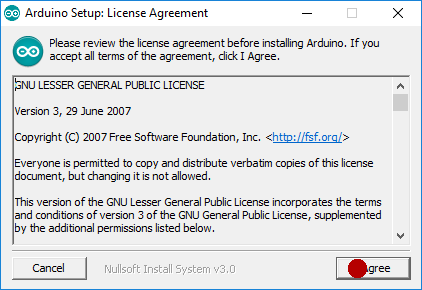
\includegraphics[width=0.9\textwidth]{figures/aride1.png}}
\item Selanjutnya akan muncul jendela `Arduino Setup: Installation Options'. Centang semua opsi yang ada, lalu klik `Next'.
\break
\centerline{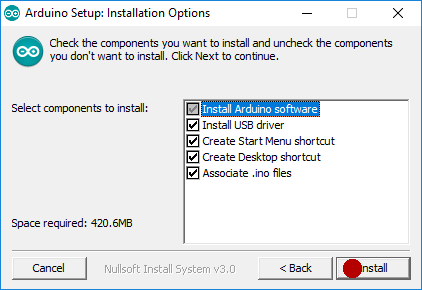
\includegraphics[width=0.9\textwidth]{figures/aride2.png}}
\item Setelah itu, akan muncul jendela `Arduino Setup: Installation Folder'. Kita diminta memilih folder instalasi Arduino.
\break
\centerline{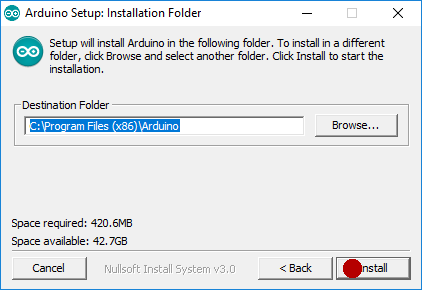
\includegraphics[width=0.9\textwidth]{figures/aride3.png}}
\item Selanjutnya proses instalasi akan dimulai.
\break
\centerline{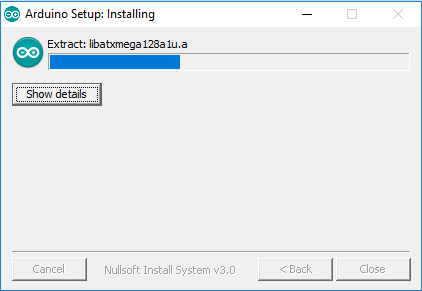
\includegraphics[width=0.9\textwidth]{figures/aride4.png}}
\item Pada saat melakukan proses instalasi, akan muncul jendela `Windows Security'. Jendela tersebut muncul apabila komputer kita belum terinstal driver - driver yang diperlukan. Klik tombol `Install'.
\break
\centerline{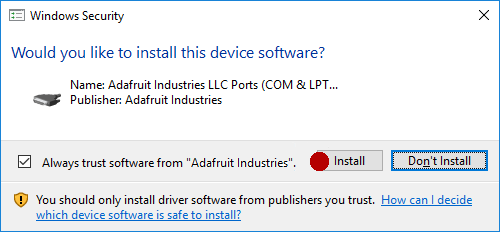
\includegraphics[width=0.9\textwidth]{figures/aride5.png}}
\break
\centerline{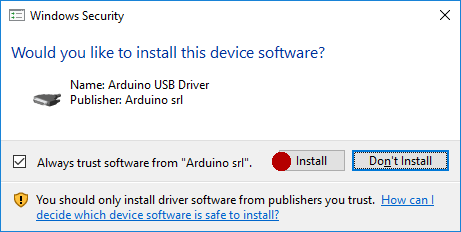
\includegraphics[width=0.9\textwidth]{figures/aride6.png}}
\break
\centerline{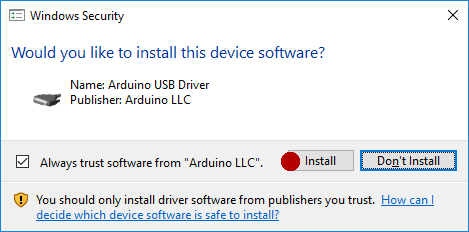
\includegraphics[width=0.9\textwidth]{figures/aride7.png}}
\item Selanjutnnya akan muncul jendela `Arduino Setup: Completed'. Jendela ini menandakan proses instalasi telah selesai. Klik tombol `Close'.
\break
\centerline{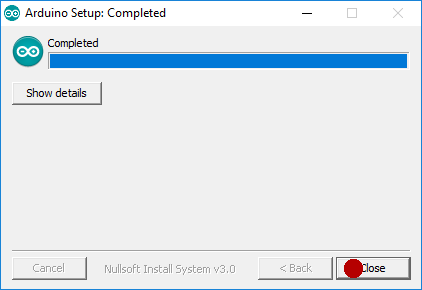
\includegraphics[width=0.9\textwidth]{figures/aride10.png}}
\item Setelah software IDE Arduino sudah terinstal. Coba cek di Start Menu Windows atau di desktop Anda, lalu jalankan aplikasi tersebut. Kemudian akan muncul splash screen seperti gambar di bawah ini.
\break
\centerline{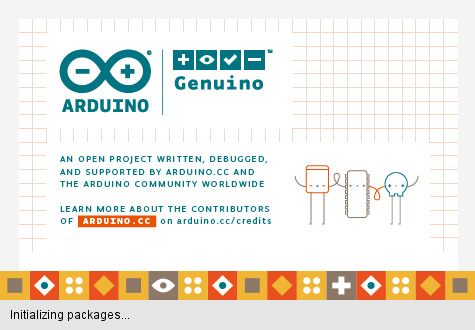
\includegraphics[width=0.9\textwidth]{figures/aride11.png}}
\item Selanjutnya akan muncul jendela IDE Arduino. Selamat Anda telah berhasil menginstal software IDE Arduino.
\break
\centerline{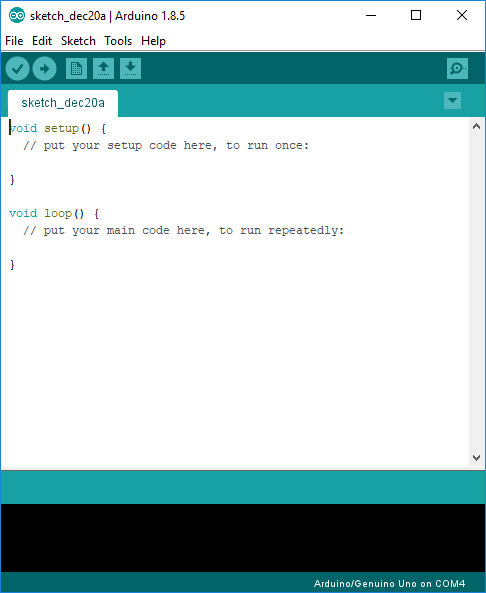
\includegraphics[width=0.9\textwidth]{figures/aride12.png}}
\end{enumerate}

\section{Fitur-Fitur IDE Arduino}

Arduino IDE dibuat dari bahasa pemrograman Java dan dilengkapi library C/C++.  Arduino IDE ini dikembangkan dari software Processing yang dirubah menjadi Arduino IDE khusus untuk pemrograman dengan Arduino. IDE Arduino terdiri dari:

\begin{itemize}

\item Editor merupakan  jendela yang digunakan oleh pengguna untuk mengubah dan menulis suatu program atau kode – kode dalam bahasa Processing.
\item Compiler merupakan sebuah modul yang mengubah kode program (bahasa Processing) menjadi kode biner. Bagaimanapun juga sebuah microcontroller tidak akan bisa memahami bahasa. Yang bisa dipahami oleh microcontroller hanya kode biner. Itulah penyebab mengapa compiler diperlukan.
\item Uploader merupakan sebuah modul yang berisi kode - kode biner atau sketch dari komputer ke dalam memory yang ada di dalam papan Arduino.
 
\end{itemize}
 
Program yang ditulis dengan menggunakan Arduino Software (IDE) disebut sebagai sketch. Sketch ditulis dalam suatu editor teks dan disimpan dalam file dengan ekstensi .ino. Teks editor pada Arduino Software memiliki beberapa fitur seperti cutting atau paste dan seraching atau replacing sehingga memudahkan kita dalam menulis kode program.

Pada Arduino IDE, terdapat semacam message box berwarna hitam yang berfungsi untuk menampilkan status, seperti pesan error, compile, dan upload program sedangkan pada bagian bawah paling kanan Arduino IDE, menunjukan board yang terkonfigurasi beserta COM Ports yang digunakan.

\subsection{Verify}
Verify berfungsi untuk melakukan memeriksa kode - kode program yang telah kita buat apakah sudah sesuai dengan kaidah pemrograman yang ada atau belum.
\subsection{Upload}
Upload berfungsi untuk melakukan kompilasi program atau kode - kode yang telah kita buat sebelumnya menjadi bahasa yang dapat dipahami oleh mesin atau Arduino.
\subsection{New}
New berfungsi untuk membuat Sketch baru.
\subsection{Open}
Open berfungsi untuk membuka kembali sketch yang telah dibuat sebelumnya untuk dilakukan perubahan atau hanya diupload ulang ke Arduino.
\subsection{Save}
Save berfungsi untuk menyimpan Sketch yang telah kita buat.
\subsection{Serial Monitor}
Serial Monitor berfungsi untuk membuka serial monitor. Serial monitor merupakan jendela yang menampilkan data yang dipertukarkan atau dikirimkan antara sketch dengan arduino pada port serialnya. Serial Monitor ini sangat berguna apabila kita ingin melakukan debugging atau yang dipertukarkan atau dikirimkan antara sketch dengan arduino pada port serialnya. Serial Monitor ini sangat berguna apabila kita ingin melakukan debugging atau membuat suatu program tanpa menggunakan LCD pada Arduino sebagai penampil nilai. Serial monitor ini dapat digunakan untuk menampilkan nilai dari proses dan pembacaan, serta pesan error.
\subsection{File}
Di dalam tab File berisi.
\begin{itemize}
\item New berfungsi untuk membuat sketch baru dengan bare minimum yang terdiri void setup() dan void loop(). 
\item Open berfungsi untuk membuka sketch yang pernah dibuat di dalam drive.
\item Open Recent berfungsi untuk mempersingkat waktu pembukaan file atau sketch yang baru-baru ini telah dibuat.
\item Sketchbook berfungsi untuk menunjukan hirarki sketch yang kita buat termasuk struktur foldernya.
\item Example berisi contoh – contoh dari pemrograman yang telah disediakan oleh pengembang Arduino, sehingga kita dapat mempelajari program-program dari contoh yang diberikan.
\item Close berfungsi untuk menghentikan dan menutup jendela Arduino IDE.
\item Save berfungsi untuk menyimpan sketch yang diubah atau baru dibuat.
\item Save as berfungsi untuk menyimpan sketch yang sedang dikerjakan atau sketch yang sudah disimpan dengan nama yang berbeda.
\item Page Setup berfungsi untuk mengatur tampilan page pada proses pencetakan.
\item Print berfungsi untuk mengirimkan file sketch ke mesin cetak untuk dicetak.
\item Preferences disini kita dapat merubah tampilan interface IDE Arduino.
\item Quit berfungsi untuk menutup semua jendela Arduino IDE.
\end{itemize}

\subsection{Edit}
Di dalam tab Edit berisi.
\begin{itemize}
\item Undo atau Redo berfungsi untuk mengembalikan perubahan yang telah dilakukan pada Sketch beberapa langkah mundur dengan Undo dan beberapa langkah maju dengan Redo.
\item Cut berfungsi untuk meremove teks yang terpilih pada editor dan menempatkan teks tersebut pada clipboard.
\item Copy berfungsi untuk menduplikasi teks yang terpilih ke dalam editor dan menempatkan teks tersebut pada clipboard.
\item Copy for Forum berfungsi untuk melakukan copy kode dari editor dan melakukan formating agar sesuai untuk ditampilkan dalam forum, sehingga kode tersebut bisa digunakan sebagai bahan diskusi dalam forum.
\item Paste berfungsi untuk menyalin data - data yang terdapat dalam clipboard, kedalam editor.
\item Select All berfungsi untuk melakukan pemilihan kode atau teks dalam halaman editor.
\item Comment atau Uncomment berfungsi untukmemberikan atau menghilangkan tanda // pada kode atau teks, dimana tanda tersebut menjadikan suatu baris kode sebagai komen dan tidak disertakan pada tahap kompilasi.
\item Increase atau Decrease Indent berfungsi untuk mengurangi atau menambahkan indentasi pada baris kode tertentu. Indentasi adalah “tab”.
\item Find berfungsi untuk memanggil jendela window find and replace, dimana kita bisa menggunakannya untuk menemukan variabel atau kata tertentu dalam program atau menemukan serta menggantikan kata tersebut dengan kata lain.
\item Find Next berfungsi untuk menemukan kata setelahnya dari kata pertama yang berhasil ditemukan.
\item Find Previous berfungsi untuk menemukan kata sebelumnya dari kata pertama yang berhasil ditemukan.
\end{itemize}	

 
\subsection{Sketch}
Di dalam tab Sketch berisi.
\begin{itemize}
\item Verify/Compile berfungsi untuk mengecek apakah sketch yang kamu buat ada kekeliruan dari segi sintaks atau tidak. Jika tidak  ada kesalahan, maka sintaks yang kamu buat akan dikompile kedalam bahasa mesin.
\item Upload berfungsi mengirimkan program yang sudah dikompilasi ke Arduino Board.
\item Uplad Using Programmer menu ini berfungsi untuk menuliskan bootloader kedalam IC Mikrokontroler Arduino. Pada kasus ini kamu membutuhkan perangkat tambahan seperti USBAsp untuk menjembatani penulisan program bootloader ke IC Mikrokontroler.
\item Export Compiled Binary berfungsi untuk menyimpan file dengan ekstensi .hex, dimana file ini dapat disimpan sebagai arsip untuk di upload ke board lain menggunakan tools yang berbeda.
\item Show Sketch Folder, berfungsi membuka folder sketch yang saat ini dikerjakan.
\item Include Library, berfunsi menambahkan library/pustaka kedalam sketch yang dibuat dengan menyertakan sintaks \#include di awal kode. Selain itu kamu juga bisa menambahkan library eksternal dari file .zip kedalam Arduino IDE.
\item Add File…, berfungsi untuk menambahkan file kedalam sketch arduino (file akan dikopikan dari drive asal). 
File akan muncul sebagai tab baru dalam jendela sketch.
\end{itemize}
 
\subsection{Tools}
Di dalam tab Tools berisi.
\begin{itemize}
\item Auto Format, berfungsi melakukan pengatran format kode pada jendela editor
\item Archive Sketch, berfungsi menyimpan sketch kedalam file .zip
\item Fix Encoding \& Reload, berfungsi memperbaiki kemungkinan perbedaan antara pengkodean peta karakter editor danpeta karakter sistem operasi yang lain.
\item Serial Monitor, berungsi membuka jendela serial monitor untuk melihat pertukaran data.
\item Board, berfungsi memilih dan melakukan konfigurasi board yang digunakan.
\item Port, memilih port sebbagai kanal komunikasi antara software dengan hardware.
\item Programmer, menu ini digunakan ketika kamu hendak melakukan pemrograman chip mikrokontroller tanpa menggunakan koneksi Onboard USB-Serial.  Biasanya digunakan pada proses burning bootloader.
\item Burn Bootloader, mengizinkan kamu untuk mengkopikan program bootloader kedalam IC mikrokontroler.
\end{itemize}

\subsection{Help}
Disini kamu bisa mendapatkan bantuan terhadap kegalauanmu mengenai pemrograman. Menu help berisikan file-file dokumentasi yang berkaitan dengan masalah yang sering muncul, serta penyelesaiannya. Selain itu pada menu help juga diberikan link untuk menuju Arduino Forum guna menanyakan serta mendiskusikan berbagai masalah yang ditemukan.

\subsection{Sketchbook}
Arduino Software IDE, menggunakan konsep sketchbook, dimana sketchbook menjadi standar peletakan dan penyimpanan file program. Sketch yang telah kamu buat dapat dibuka dengan dari File - Sketchbook, atau dengan menu Open.

\subsection{Tabs, Multiple Files, dan Compilations}
Mekanisme ini mengijinkan kamu untuk melakukan menejemen sketch, dimana lebih dari satu file dibuka dalam tab yang berbeda.

\subsection{Uploading}
Merupakan mekanisme untuk mengkopikan file .hex atau file hasil kompilasi kedalam IC mikrokontroler Arduino. Sebelum melakukan uploading, yang perlu kamu pastikan adalah jenis board yang kamu gunakan dan COM Ports dimana keduanya terletak pada menu Tools - Board dan Tools - Port.

\subsection{Library}
Library/ Pustaka merupakan file yang memberikan fungsi ekstra dari sketch yang kamu buat, semisal agar Arduino dapat bekerja dengan hardware tertentu dan melakukan proses manipulasi data. Untuk menginstal Library pihak ketiga alias Librarybukan dari Arduino, dapat dilakukan dengan Library Manager, Import file .zip, atau kopi paste secara manual di folder libraries pada Documents di platform Windows.